\documentclass[a4paper]{article}

\usepackage[english]{babel}
\usepackage[utf8]{inputenc}
\usepackage{amsmath}
\usepackage{graphicx}
\usepackage[colorinlistoftodos]{todonotes}
\usepackage[T1]{fontenc}	%ADDED for << og >>
\usepackage{enumitem}		%ADDED for smaller spacing


\title{Assinment43}

\author{pebj, smot}

\date{\today}

\begin{document}
\maketitle

\section{Most appropriate component tests}
	We have chocen to make a component test of all our  subsystems facadas, this includes EventLogic, Season and AccountManagement. We are also component testing EventComponet because it is essential for transporting data in our system. We have chocen not to make stubs for EventComponent, Account og Notification, because to make the stubs work right, we would have to implement almost the same code as the original. Given that the classes are all data classes, we see nothing wrong with it.
    
\section{Integration test strategy}
   	The strategy we are using is one of the Horizontal integration testing strategies, the bottom-up strategy. Which starts with testing each component of the bottom layer individually, then uses them to test the next layer up, by integrating them in the components their uses them. Then repeat until all components are integrated and tested together. Side note test stubs are unnecessary in this strategy.\\
	In our project we start by testing Season(D) alone, then integrate D in AccountManagement(B) and do the double test B-D and the same for D in EventLogic(C), as seen in Figure \ref{fig:Model}.Last we would have like to also have tests for the UserInterface(A) subsystem but we didn't have time for unit tests and and the last integration test A-B-C-D.


	\begin{figure}
		\centering
		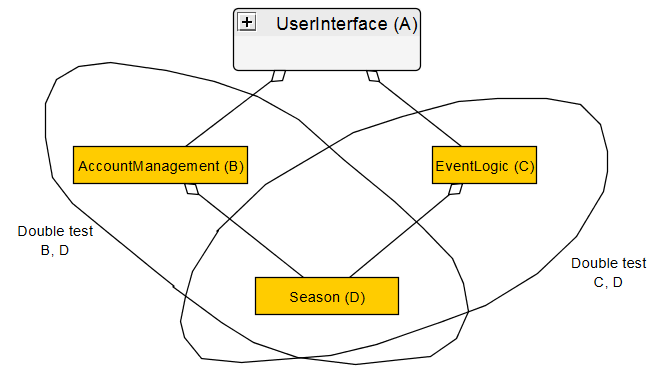
\includegraphics[width=1\textwidth]{UMLtestDiagram.PNG}\\
		\caption{Bottom-up test strategy. After unit testing subsystems B, C and D, the bottom up integration 
			test proceeds with the double tests B-D and C-D.}
		\label{fig:Model}
	\end{figure}


\end{document}